\begin{figure}[t]
\centering
\def\figwidth{0.48\columnwidth}
\begin{tabular}{@{}c c@{}}
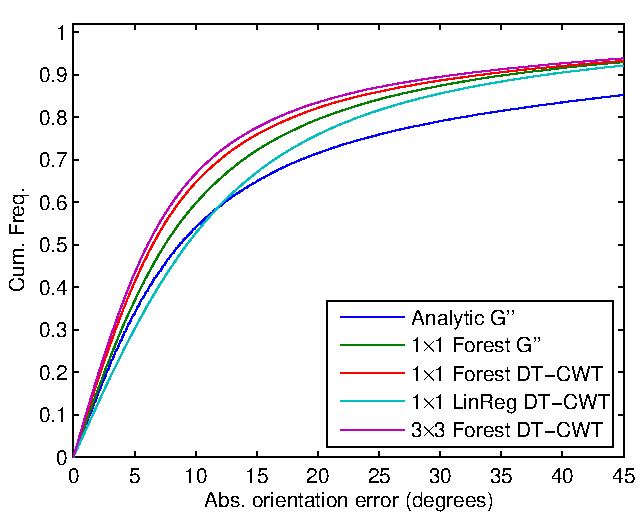
\includegraphics[width=\figwidth]{\figpath/retina/cumfreq} &
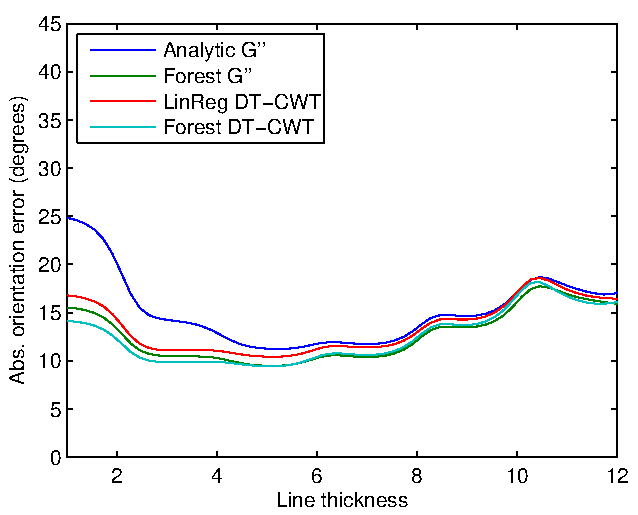
\includegraphics[width=\figwidth]{\figpath/retina/thickness_vs_error-summ} \\
(a) & (b)\\
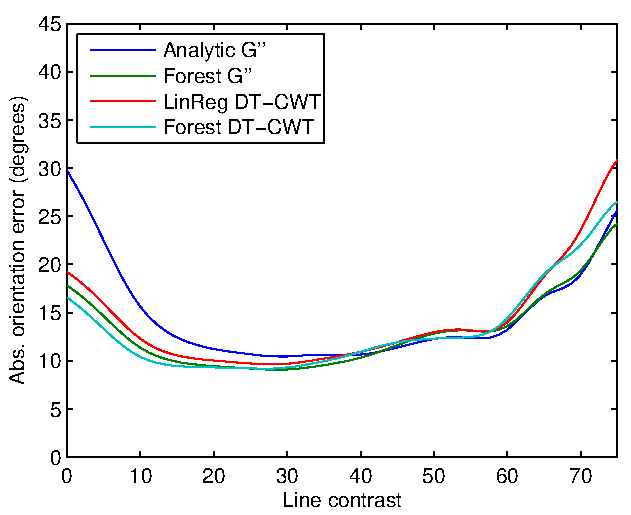
\includegraphics[width=\figwidth]{\figpath/retina/contrast_vs_error-summ} &
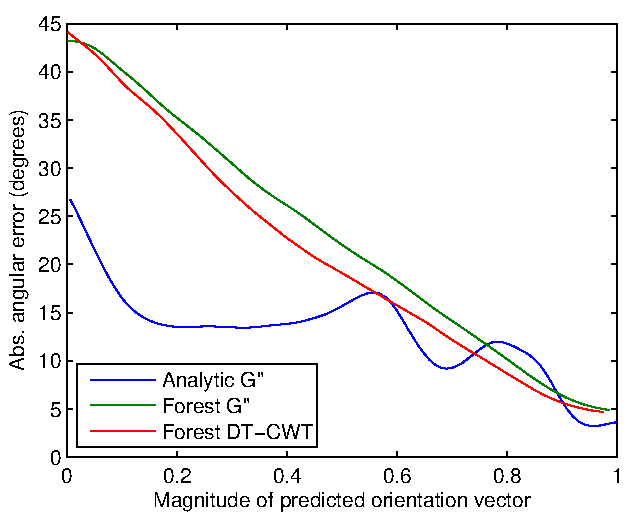
\includegraphics[width=\figwidth]{\figpath/retina/response_vs_error_ret} \\
(c) & (d)\\
\noalign{\smallskip}
\end{tabular}
%
\caption{Orientation estimation results for selected methods over pixels along the centre of the vessel: (a) Cumulative frequency of angular error; (b) Kernel estimate of mean error with respect to line thickness; (c) Kernel estimate of mean error with respect to line contrast; (d) Kernel estimate of mean error with respect to predicted orientation magnitude (for the analytic Gaussian, the absolute response scaled between 0 and 1 at the maximal angles is used).}
\label{f:retina_graphs}
\end{figure}

\comment{Some measure of spread for these figures, or a box plot to show significance.}
